\chapter{Materiais e Métodos}

\section{Modelo da rede neural DG-CA3}



Baseado nos modelos de \cite{kimAdult2024,yangDynamic2025,chavlisDendrites2017} e nos dados fisiológicos
de~\cite{wheelerHippocampomeorg2023}

A Figura~\ref{fig:arquitetura-rede} mostra a arquitetura da rede DG-CA3, ilustrando os tipos de neurônios presentes e as sinapses
existentes entre cada um.

A entrada da rede é composta pelas células do córtex entorrinal (EC, \textit{Entorhinal Cortex}),
com um total de $N_{EC} = 400$ neurônios~\cite{amaralChapter1990,kimAdult2024}.

\cite{myersRole2009, myersPattern2011}

Brian2~\cite{stimbergBrian2019a}

Runge-Kutta de 4ª ordem com passo de tempo fixo de 0,1ms~\cite{butcherHistory1996}.

\begin{figure}
    \centering
    \caption{Arquitetura da rede DG-CA3. Sinapses inibitórias são representadas por círculos e excitatórias por flechas.}
    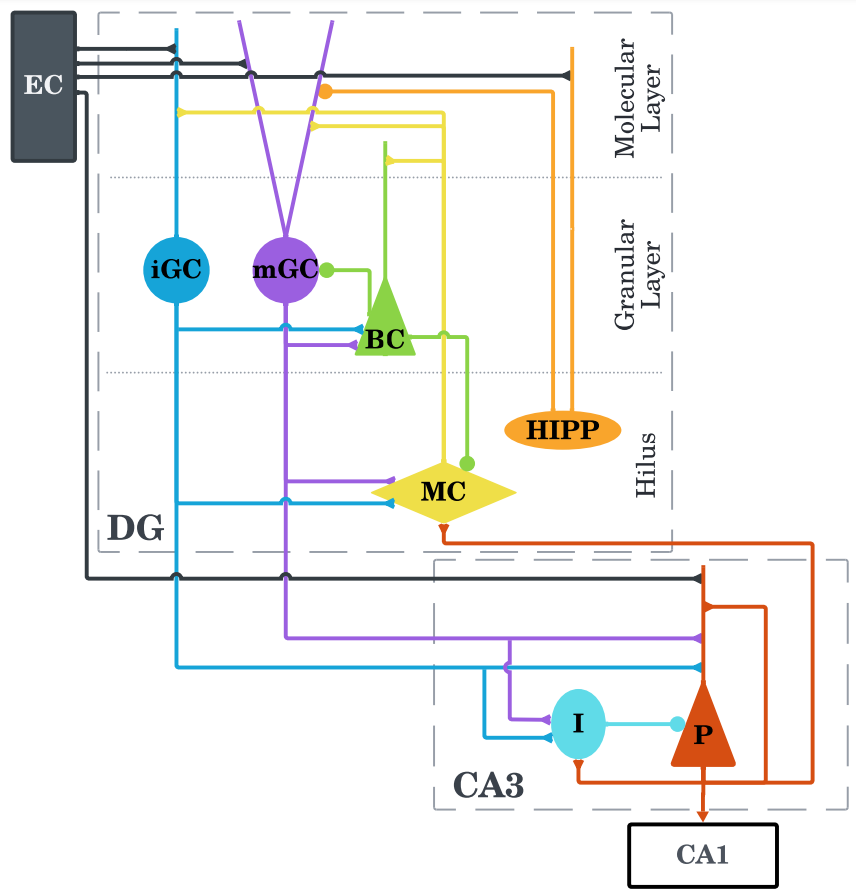
\includegraphics[width=0.9\textwidth]{figuras/arquitetura-rede.png}
    \label{fig:arquitetura-rede}
\end{figure}


\section{Modelo de neurônio}

Os neurônios foram modelados de acordo com o modelo de neurônio de Izhikevich de 9
parâmetros~\cite[cap.~8]{izhikevichDynamical2006} e um único compartimento, sem considerar dendritos ou axônios. Esse modelo foi
escolhido por ser capaz de capturar o comportamento dinâmico de neurônios em uma ampla variedade de condições com plausibilidade
biológica, como o modelo de Hodgkin-Huxley~\cite{hodgkinQuantitative1952b}, ao mesmo tempo em que apresenta um modelo matemático
mais simples e computacionalmente mais eficiente. O modelo de neurônio de Izhikevich é descrito pelas seguintes equações:

% (TODO: E por ser a escolha do Hippocampome.org)

\begin{equation}
\label{eq_izhikevich_1}
C_m \frac{dV_m}{dt} = k (V_m - V_r)(V_m - V_t) - u + I
\end{equation}

\begin{equation}
\label{eq_izhikevich_2}
\frac{du}{dt} = a [b(V_m-V_r) - u]
\end{equation}

Onde $V_m$ é o potencial de membrana, $u$ é a variável de recuperação, $C_m$ é a capacitância da membrana, $V_r$ é o
potencial de repouso, $V_t$ é o potencial de limiar, $I$ é a corrente total que flui para o neurônio e $k$, $a$ e $b$ são
constantes que definem as características dinâmicas do neurônio. Além das equações diferenciais acima, que definem a evolução
temporal do potencial de membrana e da variável de recuperação, o modelo de neurônio de Izhikevich também inclui uma regra para
a geração de potenciais de ação, definida pela equação~\ref{eq_izhikevich_3}.

\begin{equation}
\label{eq_izhikevich_3}
\text{se } V_m \geq V_{\text{peak}}, \quad
\begin{cases}
V_m \gets V_{min} \\
u \gets u + d
\end{cases}
\end{equation}

Quando o potencial de membrana atinge o valor de pico $V_{\text{peak}}$, um potencial de ação é gerado e o potencial de membrana é
redefinido para o potencial pós-disparo $V_{min}$ e a variável de recuperação $u$ é incrementada em $d$, dificultando a geração de
um próximo potencial de ação.

% Required packages: \usepackage{amsmath}, \usepackage{graphicx}, \usepackage{multirow}
\begin{table}[h!]
\centering
\renewcommand{\arraystretch}{1.4}
\resizebox{\textwidth}{!}{%
\begin{tabular}{lccccccccc}
\toprule
\multirow{2}{*}{\textbf{Célula}} & \textbf{$k$} & \textbf{$a$} & \textbf{$b$} & \textbf{$d$} & \textbf{$C_m$} & \textbf{$V_r$} & \textbf{$V_t$} & \textbf{$V_{min}$} & \textbf{$V_{peak}$} \\
 & (nS/mV) & (ms$^{-1}$) & (nS) & (pA) & (pF) & (mV) & (mV) & (mV) & (mV) \\
\midrule
$\vcenter{\hbox{
\includegraphics[height=1.5em]{figuras/neurônios/mgc.png}}}$ Granular madura & 0.45 & 0.003 & 24.48 & 50 & 38 & -77.4 & -44.9 & -66.47 & 15.49 \\
$\vcenter{\hbox{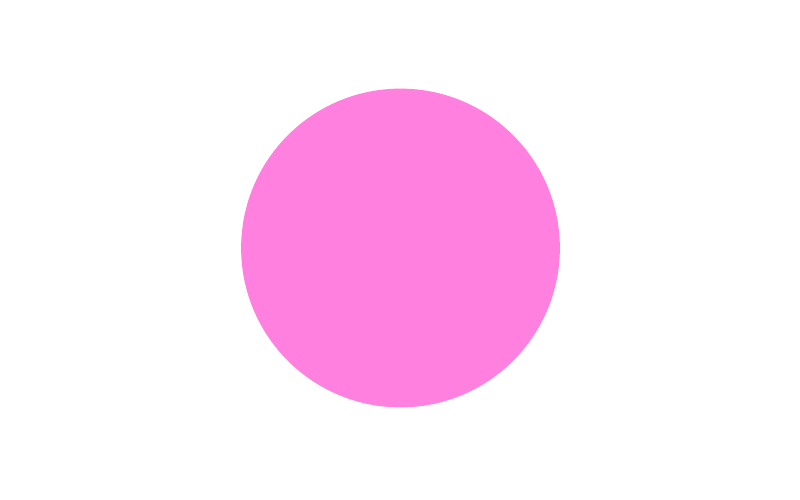
\includegraphics[height=1.5em]{figuras/neurônios/igc.png}}}$ Granular imatura & 0.139 & 0.002 & -1.877 & 12.149 & 24.6 & -63.66 & -38.41 & -48.2 & 83.5 \\
$\vcenter{\hbox{
\includegraphics[height=1.5em]{figuras/neurônios/mc.png}}}$ Musgosa & 1.5 & 0.004 & -20.84 & 117 & 258 & -63.67 & -37.11 & -47.98 & 28.29 \\
$\vcenter{\hbox{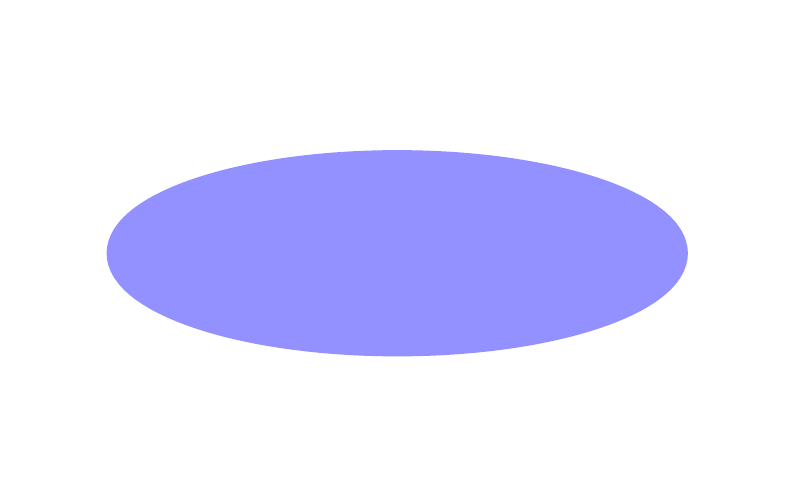
\includegraphics[height=1.5em]{figuras/neurônios/hipp.png}}}$ HIPP & 0.01 & 0.004 & -2 & 40.52 & 58.7 & -70 & -50 & -75 & 90 \\
$\vcenter{\hbox{
\includegraphics[height=1.5em]{figuras/neurônios/bc.png}}}$ Em cesto & 0.81 & 0.097 & 1.89 & 553 & 208 & -61.02 & -37.84 & -36.23 & 14.08 \\
$\vcenter{\hbox{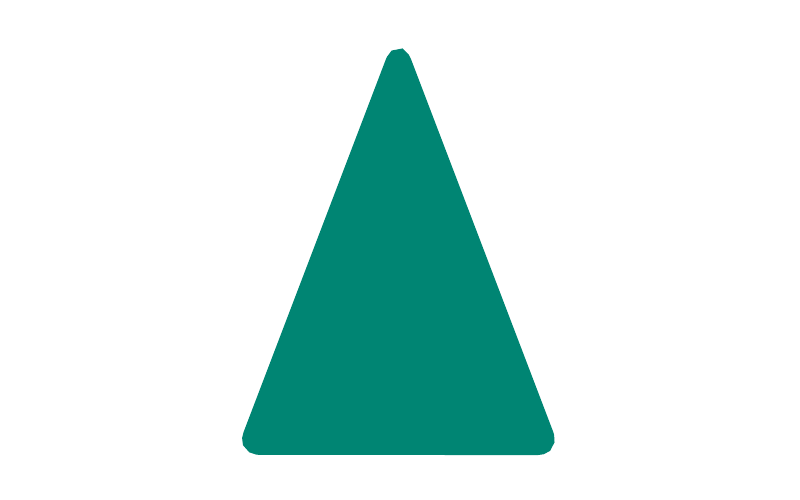
\includegraphics[height=1.5em]{figuras/neurônios/pca3.png}}}$ Piramidal do CA3 & 0.79 & 0.008 & -42.55 & 588 & 366 & -63.2 & -33.6 & -38.87 & 35.86 \\
$\vcenter{\hbox{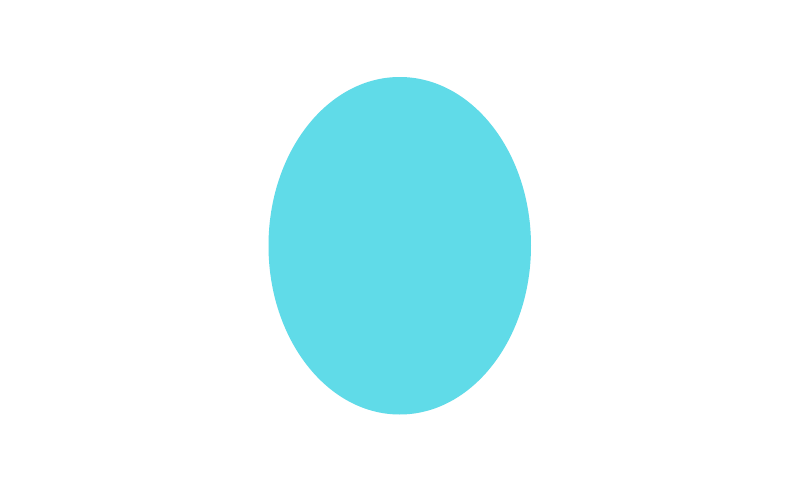
\includegraphics[height=1.5em]{figuras/neurônios/ica3.png}}}$ Inibitória do CA3 & 1 & 0.004 & 9.26 & -6 & 45 & -57.51 & -23.38 & -47.56 & 18.45 \\
\bottomrule
\end{tabular}}
\caption{Parâmetros do modelo Izhikevich por tipo de neurônio.}\label{tab:izhikevich_neuron_params}
\end{table}


\section{Modelo de sinapse}

O modelo de sinapse, assim como o de neurônio, foi definido a partir do Hippocampome.org~\cite{wheelerHippocampomeorg2023},
seguindo a formulação de~\citeonline{sennAlgorithm2001,mongilloSynaptic2008a}. Esse modelo modela a
plasticidade de curto prazo, seja ela depressão de curto prazo, causada pela depleção de neurotransmissores, ou potenciação de
curto prazo, causada pelo acúmulo de cálcio, ambas na escala dos décimos de segundos. Cada sinapse possui 5 parâmetros (descritos
na Tabela~\ref{tab:synapse_params}): a condutância máxima da sinapse no caso de nenhuma depleção de recursos sinápticos $g$, a proporção de
recursos utilizados a cada disparo $U_{se}$, a constante de tempo de decaimento da corrente sináptica $\tau_d$,
a constante de tempo de facilitação $\tau_f$, e a constante de tempo de recuperação dos recursos $\tau_r$~\cite{moradiNormalized2022}.

O modelo é descrito por três variáveis de estado: a utilização dos recursos sinápticos ($U$), a recuperação desses recursos ($R$),
inicialmente igual a 1, e a porcentagem de recursos em estado ativo ($A$). A evolução temporal dessas
variáveis é governada pelo seguinte sistema de equações diferenciais:

\begin{equation}
    \label{eq_tsodyks_dU}
    \frac{dU}{dt} = \frac{-U}{\tau_f} + U_{se}(1-U_{-}) \delta(\Delta t_i)
\end{equation}

\begin{equation}
    \label{eq_tsodyks_dR}
    \frac{dR}{dt} = \frac{1-R-A}{\tau_r} - U_{+} R_{-} \delta(\Delta t_i)
\end{equation}

\begin{equation}
    \label{eq_tsodyks_dA}
    \frac{dA}{dt} = \frac{-A}{\tau_d} + U_{+} R_{-} \delta(\Delta t_i)
\end{equation}

nde $\delta$ é a função delta de Dirac, que resulta em 1 apenas quando $\Delta t_i = t - t_i = 0$, ou seja, apenas no tempo $t$
correspondente ao tempo do evento sináptico $t_i$. $U_{+}$ corresponde ao valor de $U$ logo após o evento sináptico, enquanto que
$R_{-}$ corresponde ao valor de $R$ logo antes do mesmo.

A partir dessas equações, a corrente sináptica é dada por:

\begin{equation}
    \label{eq_tsodyks_I}
    I = k \cdot A \cdot g \cdot (V_m - E)
\end{equation}

onde $V_m$ é o potencial de membrana do neurônio pós-sináptico, $E$ é o potencial de reversão da sinapse, para sinapses
inibitórias e excitatórias, respectivamente, $E_{inh} = \SI{-86}{\milli\volt}$ e $E_{exc} = \SI{0}{\milli\volt}$, e $k$
é uma constante de escala definida como $k = 10$ para todas as sinapses. Essa constante de escala é necessária por conta
da escala reduzida da rede, visto que, pelo baixo número de sinapses do modelo comparado ao hipocampo do rato, sem o 
escalamento a rede toda ficaria silenciosa.


% Synapse Parameters Table
% Required packages: \usepackage{amsmath}, \usepackage{graphicx}, \usepackage{multirow}
\begin{table}[h!]
\centering
\renewcommand{\arraystretch}{1.4}
\resizebox{\textwidth}{!}{%
\begin{tabular}{llccccccc}
\toprule
\multirow{2}{*}{\textbf{Pré-sináptico}} & \multirow{2}{*}{\textbf{Pós-sináptico}} & \multirow{2}{*}{\textbf{Conexão}} & $P$ & \textbf{$g$} & \textbf{$\tau_d$} & \textbf{$\tau_r$} & \textbf{$\tau_f$} & \textbf{$U$} \\
 & & & (\%) & (nS) & (ms) & (ms) & (ms) &  \\
\midrule
$\vcenter{\hbox{
\includegraphics[height=1.5em]{figuras/neurônios/pp.png}}}$ Córtex Entorrinal & $\vcenter{\hbox{
\includegraphics[height=1.5em]{figuras/neurônios/mgc.png}}}$ Granular madura & Aleatória & 8 & 1.825 & 5.333 & 266.239 & 18.714 & 0.27 \\
$\vcenter{\hbox{
\includegraphics[height=1.5em]{figuras/neurônios/pp.png}}}$ Córtex Entorrinal & $\vcenter{\hbox{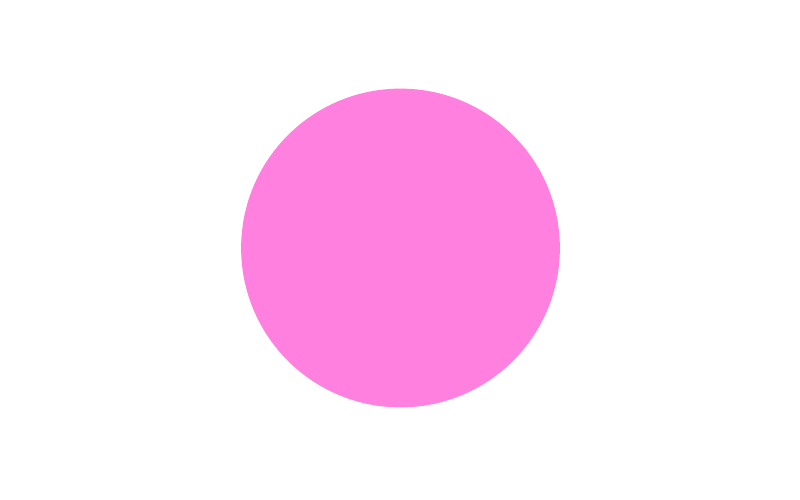
\includegraphics[height=1.5em]{figuras/neurônios/igc.png}}}$ Granular imatura & Aleatória & 8 & 1.825 & 5.333 & 266.239 & 18.714 & 0.27 \\
$\vcenter{\hbox{
\includegraphics[height=1.5em]{figuras/neurônios/pp.png}}}$ Córtex Entorrinal & $\vcenter{\hbox{
\includegraphics[height=1.5em]{figuras/neurônios/mc.png}}}$ Musgosa & Aleatória & 20 & 1.422 & 4.671 & 319.835 & 57.766 & 0.204 \\
$\vcenter{\hbox{
\includegraphics[height=1.5em]{figuras/neurônios/pp.png}}}$ Córtex Entorrinal & $\vcenter{\hbox{
\includegraphics[height=1.5em]{figuras/neurônios/bc.png}}}$ Em cesto & Aleatória & 20 & 1.406 & 3.849 & 144.415 & 48.2 & 0.214 \\
$\vcenter{\hbox{
\includegraphics[height=1.5em]{figuras/neurônios/pp.png}}}$ Córtex Entorrinal & $\vcenter{\hbox{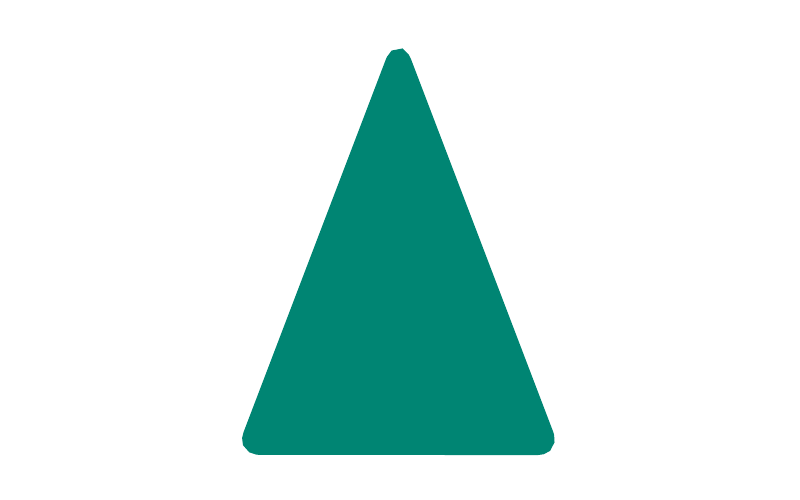
\includegraphics[height=1.5em]{figuras/neurônios/pca3.png}}}$ Piramidal do CA3 & Aleatória & 4 & 1.065 & 6.55 & 258.318 & 53.478 & 0.184 \\
$\vcenter{\hbox{
\includegraphics[height=1.5em]{figuras/neurônios/pp.png}}}$ Córtex Entorrinal & $\vcenter{\hbox{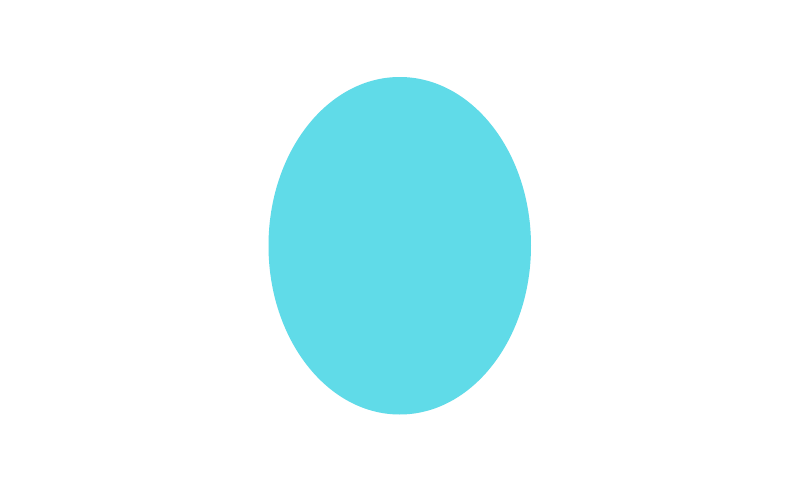
\includegraphics[height=1.5em]{figuras/neurônios/ica3.png}}}$ Inibitória do CA3 & Aleatória & 20 & 1.556 & 3.602 & 457.468 & 35.904 & 0.21 \\
$\vcenter{\hbox{
\includegraphics[height=1.5em]{figuras/neurônios/mgc.png}}}$ Granular madura & $\vcenter{\hbox{
\includegraphics[height=1.5em]{figuras/neurônios/mc.png}}}$ Musgosa & Lamelar & 20 & 1.713 & 5.347 & 428.583 & 73.479 & 0.151 \\
$\vcenter{\hbox{
\includegraphics[height=1.5em]{figuras/neurônios/mgc.png}}}$ Granular madura & $\vcenter{\hbox{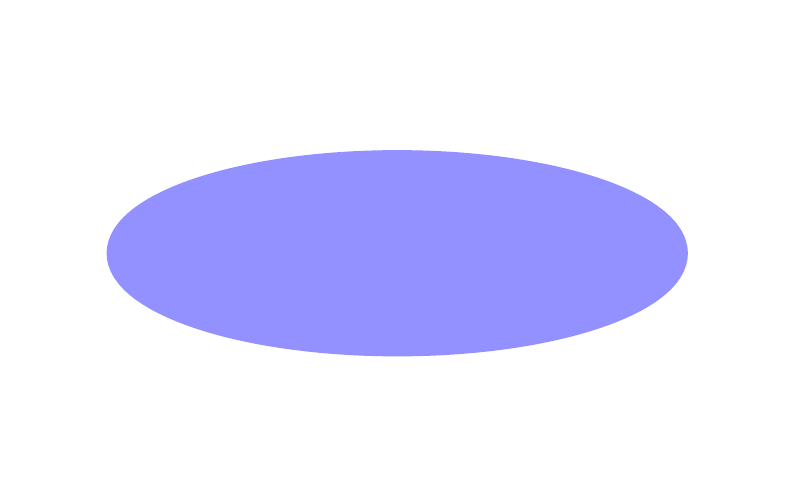
\includegraphics[height=1.5em]{figuras/neurônios/hipp.png}}}$ HIPP & Aleatória & 5 & 1.305 & 5.181 & 462.814 & 48.986 & 0.15 \\
$\vcenter{\hbox{
\includegraphics[height=1.5em]{figuras/neurônios/mgc.png}}}$ Granular madura & $\vcenter{\hbox{
\includegraphics[height=1.5em]{figuras/neurônios/bc.png}}}$ Em cesto & Lamelar & 100 & 1.458 & 3.566 & 151.265 & 62.278 & 0.197 \\
$\vcenter{\hbox{
\includegraphics[height=1.5em]{figuras/neurônios/mgc.png}}}$ Granular madura & $\vcenter{\hbox{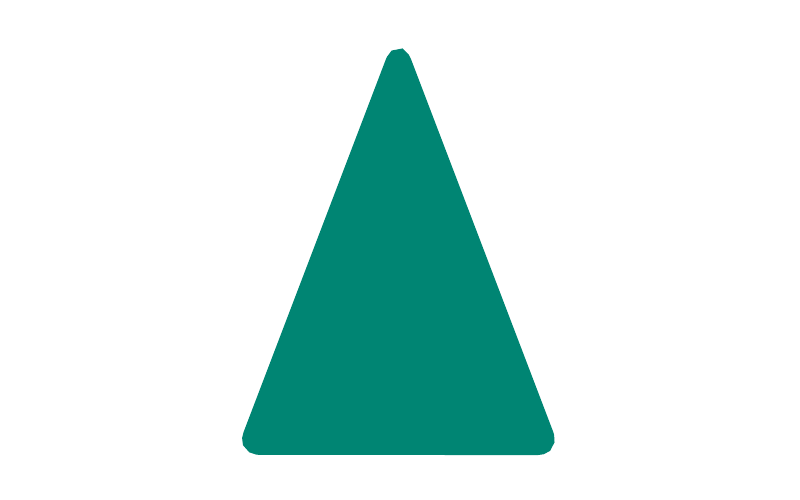
\includegraphics[height=1.5em]{figuras/neurônios/pca3.png}}}$ Piramidal do CA3 & Lamelar & 60 & 1.384 & 6.657 & 278.286 & 78.584 & 0.155 \\
$\vcenter{\hbox{
\includegraphics[height=1.5em]{figuras/neurônios/mgc.png}}}$ Granular madura & $\vcenter{\hbox{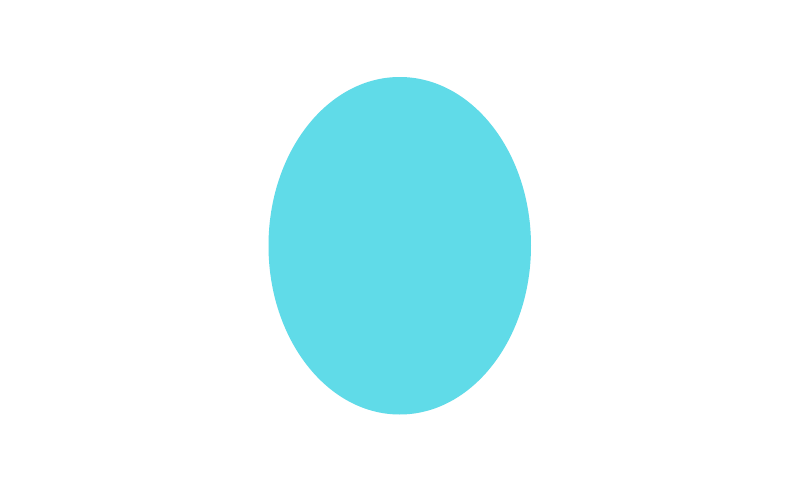
\includegraphics[height=1.5em]{figuras/neurônios/ica3.png}}}$ Inibitória do CA3 & Lamelar & 100 & 1.625 & 3.915 & 518.934 & 43.274 & 0.176 \\
$\vcenter{\hbox{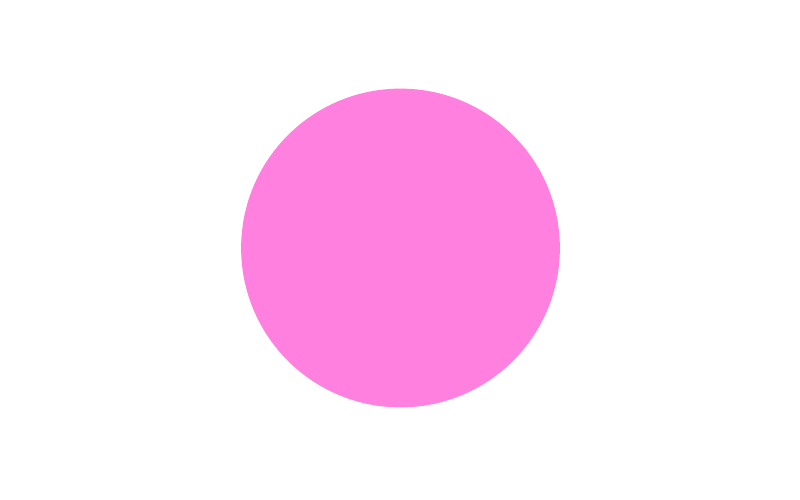
\includegraphics[height=1.5em]{figuras/neurônios/igc.png}}}$ Granular imatura & $\vcenter{\hbox{
\includegraphics[height=1.5em]{figuras/neurônios/mc.png}}}$ Musgosa & Lamelar & 20 & 1.713 & 5.347 & 428.583 & 73.479 & 0.151 \\
$\vcenter{\hbox{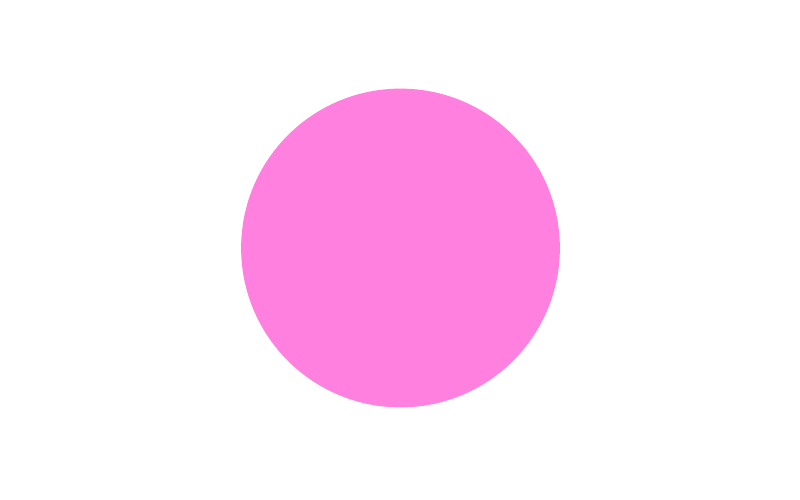
\includegraphics[height=1.5em]{figuras/neurônios/igc.png}}}$ Granular imatura & $\vcenter{\hbox{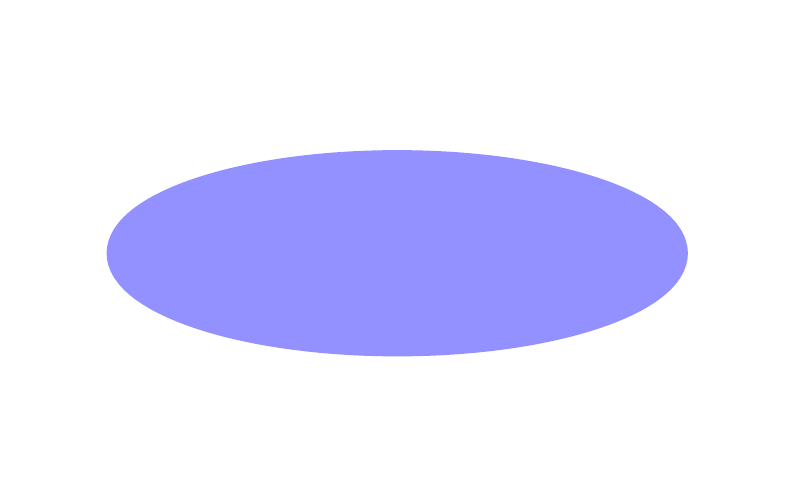
\includegraphics[height=1.5em]{figuras/neurônios/hipp.png}}}$ HIPP & Aleatória & 5 & 1.305 & 5.181 & 462.814 & 48.986 & 0.15 \\
$\vcenter{\hbox{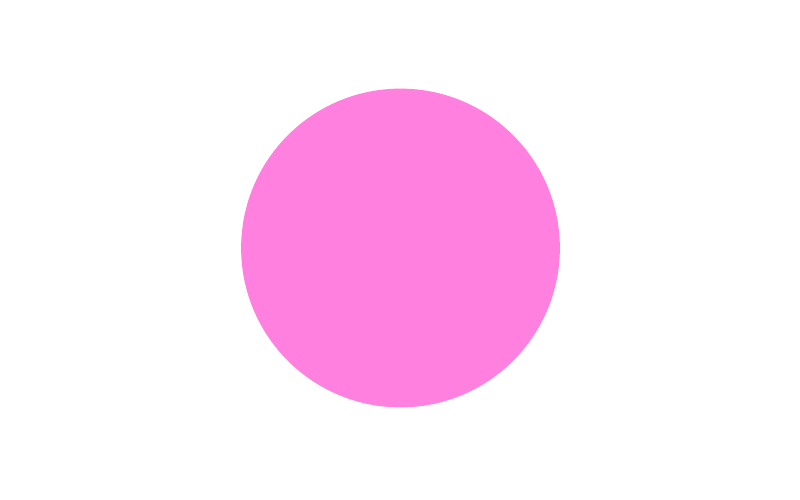
\includegraphics[height=1.5em]{figuras/neurônios/igc.png}}}$ Granular imatura & $\vcenter{\hbox{
\includegraphics[height=1.5em]{figuras/neurônios/bc.png}}}$ Em cesto & Lamelar & 100 & 1.458 & 3.566 & 151.265 & 62.278 & 0.197 \\
$\vcenter{\hbox{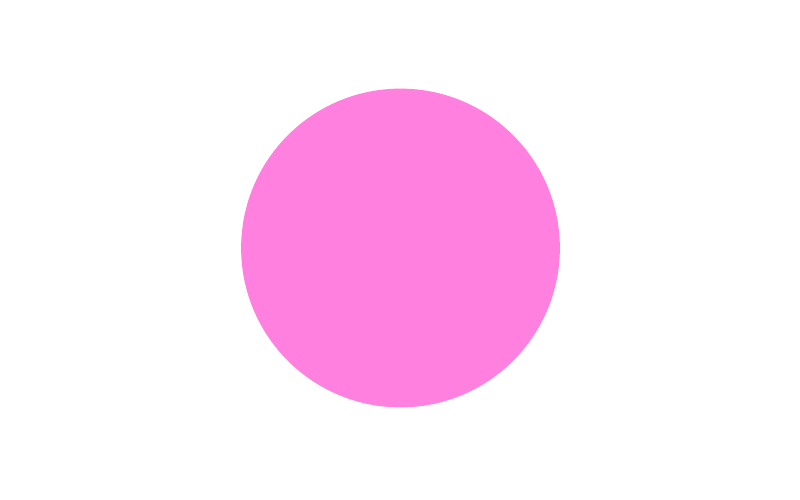
\includegraphics[height=1.5em]{figuras/neurônios/igc.png}}}$ Granular imatura & $\vcenter{\hbox{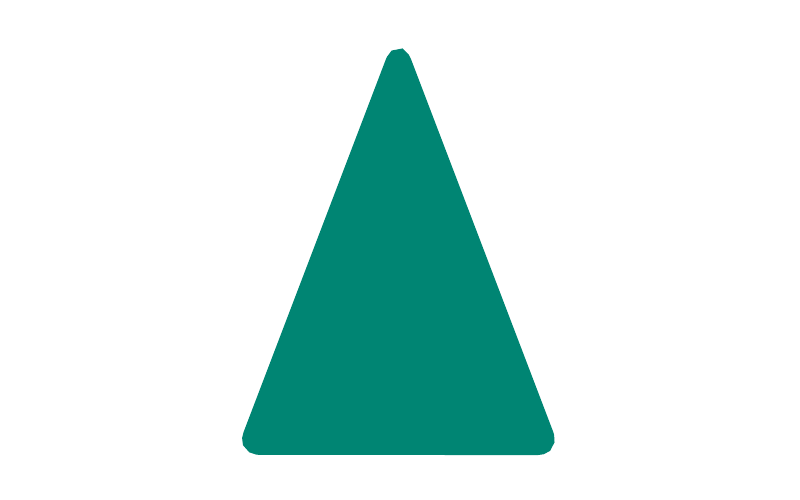
\includegraphics[height=1.5em]{figuras/neurônios/pca3.png}}}$ Piramidal do CA3 & Lamelar & 60 & 1.384 & 6.657 & 278.286 & 78.584 & 0.155 \\
$\vcenter{\hbox{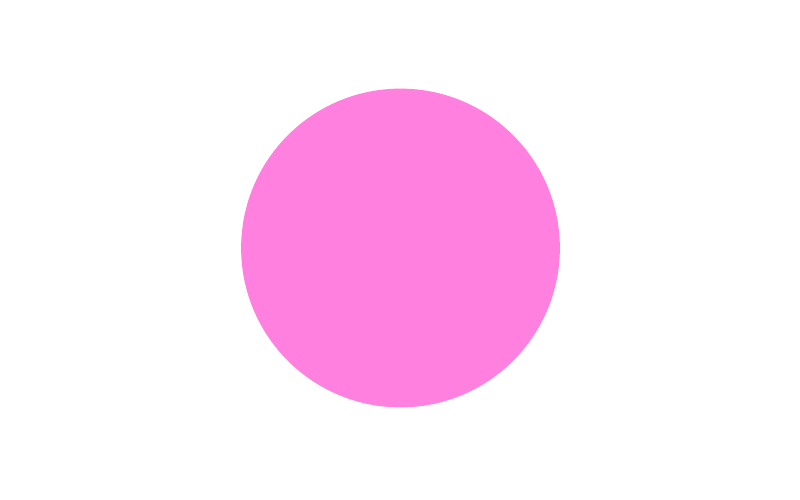
\includegraphics[height=1.5em]{figuras/neurônios/igc.png}}}$ Granular imatura & $\vcenter{\hbox{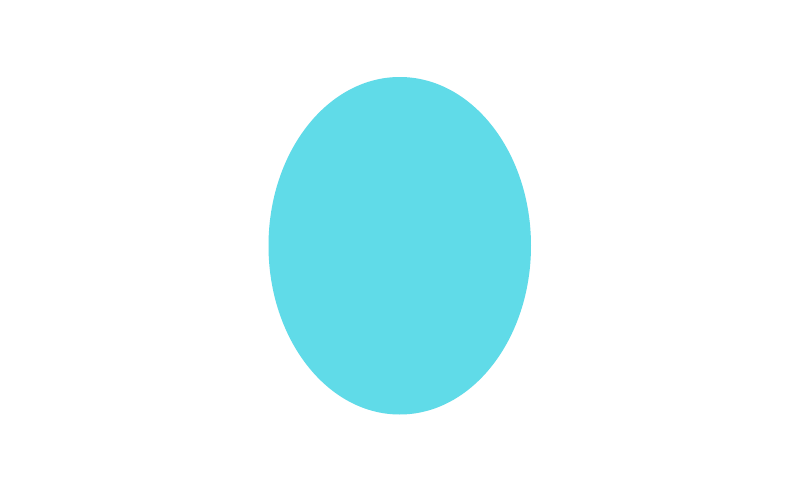
\includegraphics[height=1.5em]{figuras/neurônios/ica3.png}}}$ Inibitória do CA3 & Lamelar & 100 & 1.625 & 3.915 & 518.934 & 43.274 & 0.176 \\
$\vcenter{\hbox{
\includegraphics[height=1.5em]{figuras/neurônios/mc.png}}}$ Musgosa & $\vcenter{\hbox{
\includegraphics[height=1.5em]{figuras/neurônios/mgc.png}}}$ Granular madura & Interlamelar & 0.2 & 2.394 & 5.357 & 166.162 & 20.224 & 0.304 \\
$\vcenter{\hbox{
\includegraphics[height=1.5em]{figuras/neurônios/mc.png}}}$ Musgosa & $\vcenter{\hbox{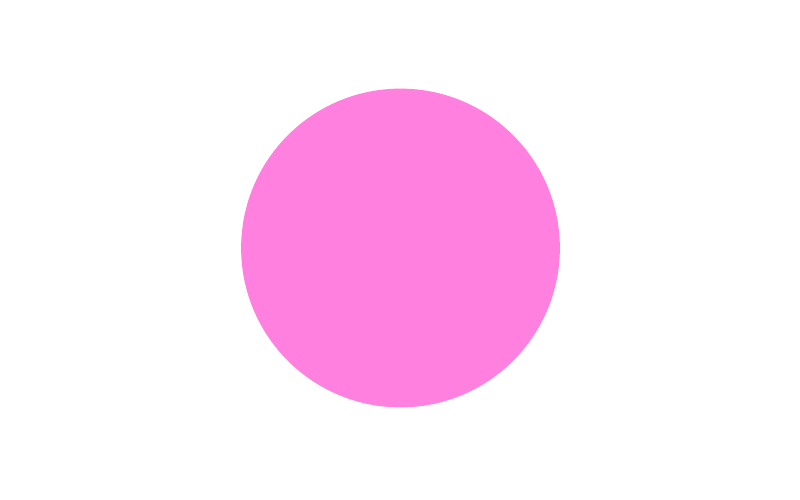
\includegraphics[height=1.5em]{figuras/neurônios/igc.png}}}$ Granular imatura & Interlamelar & 0.2 & 2.394 & 5.357 & 166.162 & 20.224 & 0.304 \\
$\vcenter{\hbox{
\includegraphics[height=1.5em]{figuras/neurônios/mc.png}}}$ Musgosa & $\vcenter{\hbox{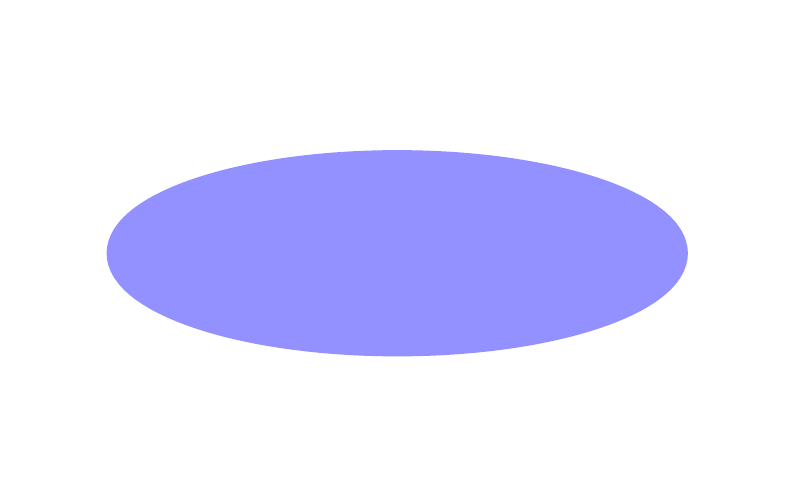
\includegraphics[height=1.5em]{figuras/neurônios/hipp.png}}}$ HIPP & Interlamelar & 100 & 1.376 & 4.824 & 358.431 & 54.872 & 0.181 \\
$\vcenter{\hbox{
\includegraphics[height=1.5em]{figuras/neurônios/mc.png}}}$ Musgosa & $\vcenter{\hbox{
\includegraphics[height=1.5em]{figuras/neurônios/bc.png}}}$ Em cesto & Interlamelar & 100 & 1.996 & 3.396 & 117.365 & 69.316 & 0.255 \\
$\vcenter{\hbox{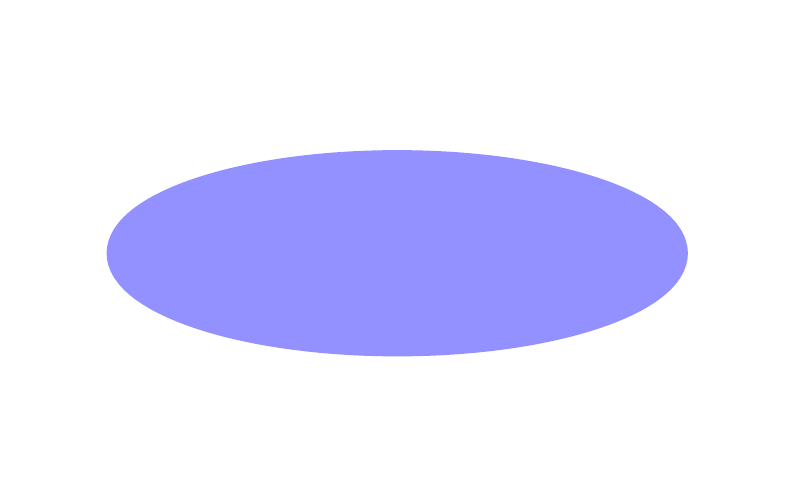
\includegraphics[height=1.5em]{figuras/neurônios/hipp.png}}}$ HIPP & $\vcenter{\hbox{
\includegraphics[height=1.5em]{figuras/neurônios/mgc.png}}}$ Granular madura & Aleatória & 20 & 2.002 & 8.935 & 559.143 & 8.396 & 0.278 \\
$\vcenter{\hbox{\includegraphics[height=1.5em]{figuras/neurônios/hipp.png}}}$ HIPP & $\vcenter{\hbox{\includegraphics[height=1.5em]{figuras/neurônios/igc.png}}}$ Granular imatura & Aleatória & 10 & 2.002 & 8.935 & 559.143 & 8.396 & 0.278 \\
$\vcenter{\hbox{\includegraphics[height=1.5em]{figuras/neurônios/hipp.png}}}$ HIPP & $\vcenter{\hbox{\includegraphics[height=1.5em]{figuras/neurônios/bc.png}}}$ Em cesto & Aleatória & 2 & 1.709 & 5.982 & 367.198 & 15.292 & 0.221 \\
$\vcenter{\hbox{\includegraphics[height=1.5em]{figuras/neurônios/bc.png}}}$ Em cesto & $\vcenter{\hbox{\includegraphics[height=1.5em]{figuras/neurônios/mgc.png}}}$ Granular madura & Lamelar & 100 & 2.451 & 6.543 & 433.876 & 6.347 & 0.332 \\
$\vcenter{\hbox{\includegraphics[height=1.5em]{figuras/neurônios/bc.png}}}$ Em cesto & $\vcenter{\hbox{\includegraphics[height=1.5em]{figuras/neurônios/igc.png}}}$ Granular imatura & Lamelar & 100 & 2.451 & 6.543 & 433.876 & 6.347 & 0.332 \\
$\vcenter{\hbox{\includegraphics[height=1.5em]{figuras/neurônios/bc.png}}}$ Em cesto & $\vcenter{\hbox{\includegraphics[height=1.5em]{figuras/neurônios/hipp.png}}}$ HIPP & Aleatória & 2 & 1.408 & 6.544 & 534.182 & 8.385 & 0.24 \\
$\vcenter{\hbox{\includegraphics[height=1.5em]{figuras/neurônios/pca3.png}}}$ Piramidal do CA3 & $\vcenter{\hbox{\includegraphics[height=1.5em]{figuras/neurônios/pca3.png}}}$ Piramidal do CA3 & Aleatória & 2 & 0.603 & 9.516 & 278.258 & 27.513 & 0.172 \\
$\vcenter{\hbox{\includegraphics[height=1.5em]{figuras/neurônios/pca3.png}}}$ Piramidal do CA3 & $\vcenter{\hbox{\includegraphics[height=1.5em]{figuras/neurônios/mc.png}}}$ Musgosa & Lamelar & 10 & 2.035 & 4.297 & 359.116 & 40.457 & 0.236 \\
$\vcenter{\hbox{\includegraphics[height=1.5em]{figuras/neurônios/pca3.png}}}$ Piramidal do CA3 & $\vcenter{\hbox{\includegraphics[height=1.5em]{figuras/neurônios/ica3.png}}}$ Inibitória do CA3 & Aleatória & 100 & 1.247 & 4.525 & 525.605 & 23.321 & 0.189 \\
$\vcenter{\hbox{\includegraphics[height=1.5em]{figuras/neurônios/ica3.png}}}$ Inibitória do CA3 & $\vcenter{\hbox{\includegraphics[height=1.5em]{figuras/neurônios/pca3.png}}}$ Piramidal do CA3 & Aleatória & 100 & 1.462 & 7.793 & 416.282 & 20.63 & 0.203 \\
\bottomrule
\end{tabular}}
\caption{Parâmetros das sinapses entre as populações neuronais. Conexões aleatórias ocorrem entre todas as células
              de ambas as populações; conexões lamelares ocorrem entre células da mesma lamela; conexões interlamelares ocorrem
              entre as células de uma lamela com todas as demais. A probabilidade de conexão $P$ diz respeito à porcentagem de
              conexões entre as populações neuronais de acordo com a condição de conexão.}
\label{tab:synapse_params}
\end{table}



\section{Plasticidade de longo prazo}

\section{Neurogênese temporal}

\section{Separação de padrões}

A metodologia para quantificar a separação de padrões foi baseada na que foi utilizada em~\cite{kimEffect2024}.
Para caracterizar a separação de padrões, é comparada a sobreposição entre os padrões de atividade neural na entrada (células do
córtex entorrinal) e na saída (células granulares do DG, ou piramidais do CA3) da rede. Um padrão é definido por um
representação binária de tamanho $N$, onde $N$ é o número total de neurônios de uma população específica, em que neurônios que
dispararam ao menos uma vez durante o intervalo de tempo da simulação são representados por 1 e os que não dispararam são
representados por 0. Para um par de padrões $A^{(l)}$ e $B^{(l)}$ (onde $l \in \{in, out\}$ para entrada e saída,
respectivamente), a distância entre os padrões $D_p^{(l)}$ é definida como:

\begin{equation}
    \label{eq:dp}
    D_p^{(l)} = \frac{O^{(l)}}{D_a^{(l)}}
\end{equation}

Nesta equação, $O^{(l)}$ representa o grau de ortogonalização e $D_a^{(l)}$ o grau médio de ativação dos dois padrões. O grau médio de ativação $D_a^{(l)}$ é a média aritmética dos graus de ativação de cada padrão, $A^{(l)}$ e $B^{(l)}$:

\begin{equation}
    \label{eq:da}
    D_a^{(l)} = \frac{D_a^{(A^{(l)})} + D_a^{(B^{(l)})}}{2}
\end{equation}

O grau de ativação de um padrão individual é a fração de neurônios ativos (representados por 1 em uma codificação binária) no padrão.
O grau de ortogonalização $O^{(l)}$, que mede a dissimilaridade entre os padrões, é calculado a partir do coeficiente de correlação de Pearson, $\rho^{(l)}$:

\begin{equation}
    \label{eq:o}
    O^{(l)} = \frac{1 - \rho^{(l)}}{2}
\end{equation}

Onde $\rho^{(l)}$ é o coeficiente de correlação de Pearson entre os padrões $A^{(l)}$ e $B^{(l)}$.
Considerando $\{a_i^{(l)}\}$ e $\{b_i^{(l)}\}$ ($i=1, \dots, N_l$) como as representações binárias do estado da $i$-ésima célula nos padrões $A^{(l)}$ e $B^{(l)}$ ($l \in \{in, out\}$), o coeficiente de correlação de Pearson é dado por:

\begin{equation}
    \label{eq:pearson}
    \rho^{(l)} = \frac{\sum_{i=1}^{N_l} \Delta a_i^{(l)} \cdot \Delta b_i^{(l)}}{\sqrt{\sum_{i=1}^{N_l} (\Delta a_i^{(l)})^2} \sqrt{\sum_{i=1}^{N_l} (\Delta b_i^{(l)})^2}}
\end{equation}

em que $\Delta a_i^{(l)} = a_i^{(l)} - \langle a^{(l)} \rangle$ e $\Delta b_i^{(l)} = b_i^{(l)} - \langle b^{(l)} \rangle$. A notação $\langle \dots \rangle$ indica a média populacional sobre todas as células. O valor de $\rho^{(l)}$ varia entre -1 e 1.
A similaridade entre os padrões, $C^{(l)}$, é diretamente o coeficiente de correlação de Pearson:

\begin{equation}
    \label{eq:c}
    C^{(l)} = \rho^{(l)}
\end{equation}

A partir das distâncias dos padrões de entrada ($D_p^{(in)}$) e saída ($D_p^{(out)}$), o grau de separação de padrões, $S_d$, é calculado como a razão entre elas:

\begin{equation}
    \label{eq:sd}
    S_d = \frac{D_p^{(out)}}{D_p^{(in)}}
\end{equation}

Um valor de $S_d > 1$ indica que os padrões de saída são mais distintos que os de entrada, caracterizando a separação de padrões. Inversamente, $S_d < 1$ indica uma convergência de padrões, onde os padrões de saída se tornam mais similares entre si.




